\documentclass[aspectratio=169]{beamer}
\usepackage[normalem]{ulem}


\usepackage{../theme/flagbot}
\usepackage{pgfpages}

%\setbeameroption{show notes on second screen}

\tikzstyle{freecell}=[fill=none]

\newcommand{\reg}[1]{\%\mintinline{asm}{#1}}
\newcommand{\hex}[1]{\mintinline{python}{0x#1}}
\newcommand{\naddr}[2]{\begin{tabular}{l}#1\\\hex{#2}\end{tabular}}
\newcommand{\docl}[1]{(\textbf{\href{#1}{Documentation}})}

\hypersetup{colorlinks,linkcolor=,urlcolor=brightblue}

\setbeamertemplate{navigation symbols}{}

\showsectionframe

%%%%%%%%%%%%%%%%%%%%%%%%%%%%%%%%%%%%%%%%%%%%%%%%%%%%%%%%%%%%%%%%%%%%%%%%%%%%%%%
% Title Setup
%%%%%%%%%%%%%%%%%%%%%%%%%%%%%%%%%%%%%%%%%%%%%%%%%%%%%%%%%%%%%%%%%%%%%%%%%%%%%%%
\title{\texttt{void* joinPolygl0ts()}}
\subtitle{and learn how to become a hackeAAAAAAAAAAAAAAAAØ·!'Ëêõá|æ}
\author{Solene Husseini \and Florian Hofhammer}
\date{\today}
\begin{document}  
\titleframe

\begin{frame}
    \frametitle{About polygl0ts}
    \begin{columns}
        \begin{column}{0.5\textwidth}
            \begin{itemize}
                \item Formed in 2018
				\item High rankings in numerous ctfs
				\item \#1 in Switzerland in 2022
				\item Still going strong
            \end{itemize}
        \end{column}
        \begin{column}{0.5\textwidth}
            \begin{tikzpicture}
                \begin{scope}
                  \node [inner sep=0pt] (0,0) (image) {
\includegraphics[width=3cm]{../theme/FlagbotBotOnly.png}};
                \end{scope}
                \node[align=center, anchor=north] at (image.south) {More Information: \href{https://polygl0ts.ch}{\UrlFont{polygl0ts.ch}}};
              \end{tikzpicture}
            
        \end{column}
    \end{columns}
\end{frame}

\begin{frame}
	\frametitle{What even is a CTF?}
	\begin{itemize}
		\item \textit{Capture the Flag} competitions
	\end{itemize}
	\pause
	\vspace{2em}
	As with many computer science terms, like:
	\begin{itemize}
		\item shebang
		\item man touch
		\item latex strip commands
		\item python internals
	\end{itemize}
	You should avoid googling it right away...
\end{frame}

\begin{frame}
	\frametitle{What even is a CTF?}
	\begin{center}
	\begin{tikzpicture}
		\begin{scope}
			\node (0,0) (image) {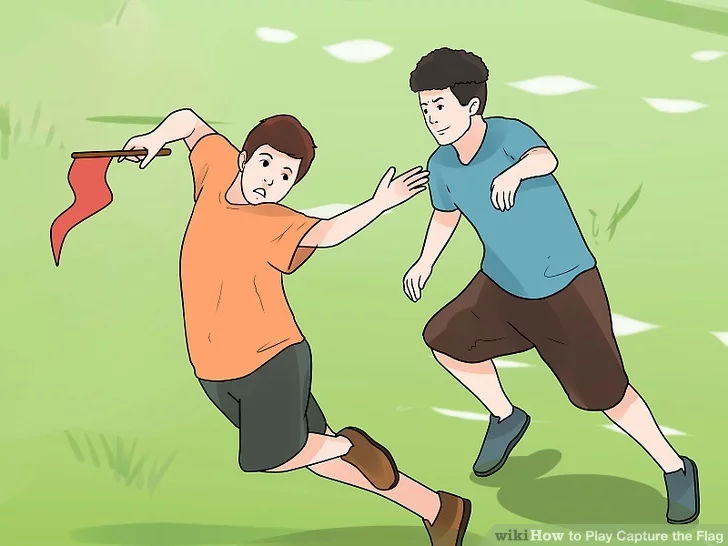
\includegraphics[scale=0.3]{./capture_the_flag.png}};
		\end{scope}
		\node[align=center, anchor=north] at (image.south) {Don't google it -- it's not this};
	\end{tikzpicture}
	\end{center}
\end{frame}

\begin{frame}
	\frametitle{What even is a CTF?}
	\begin{center}
	\begin{tikzpicture}
		\begin{scope}
			\node (0,0) (image) {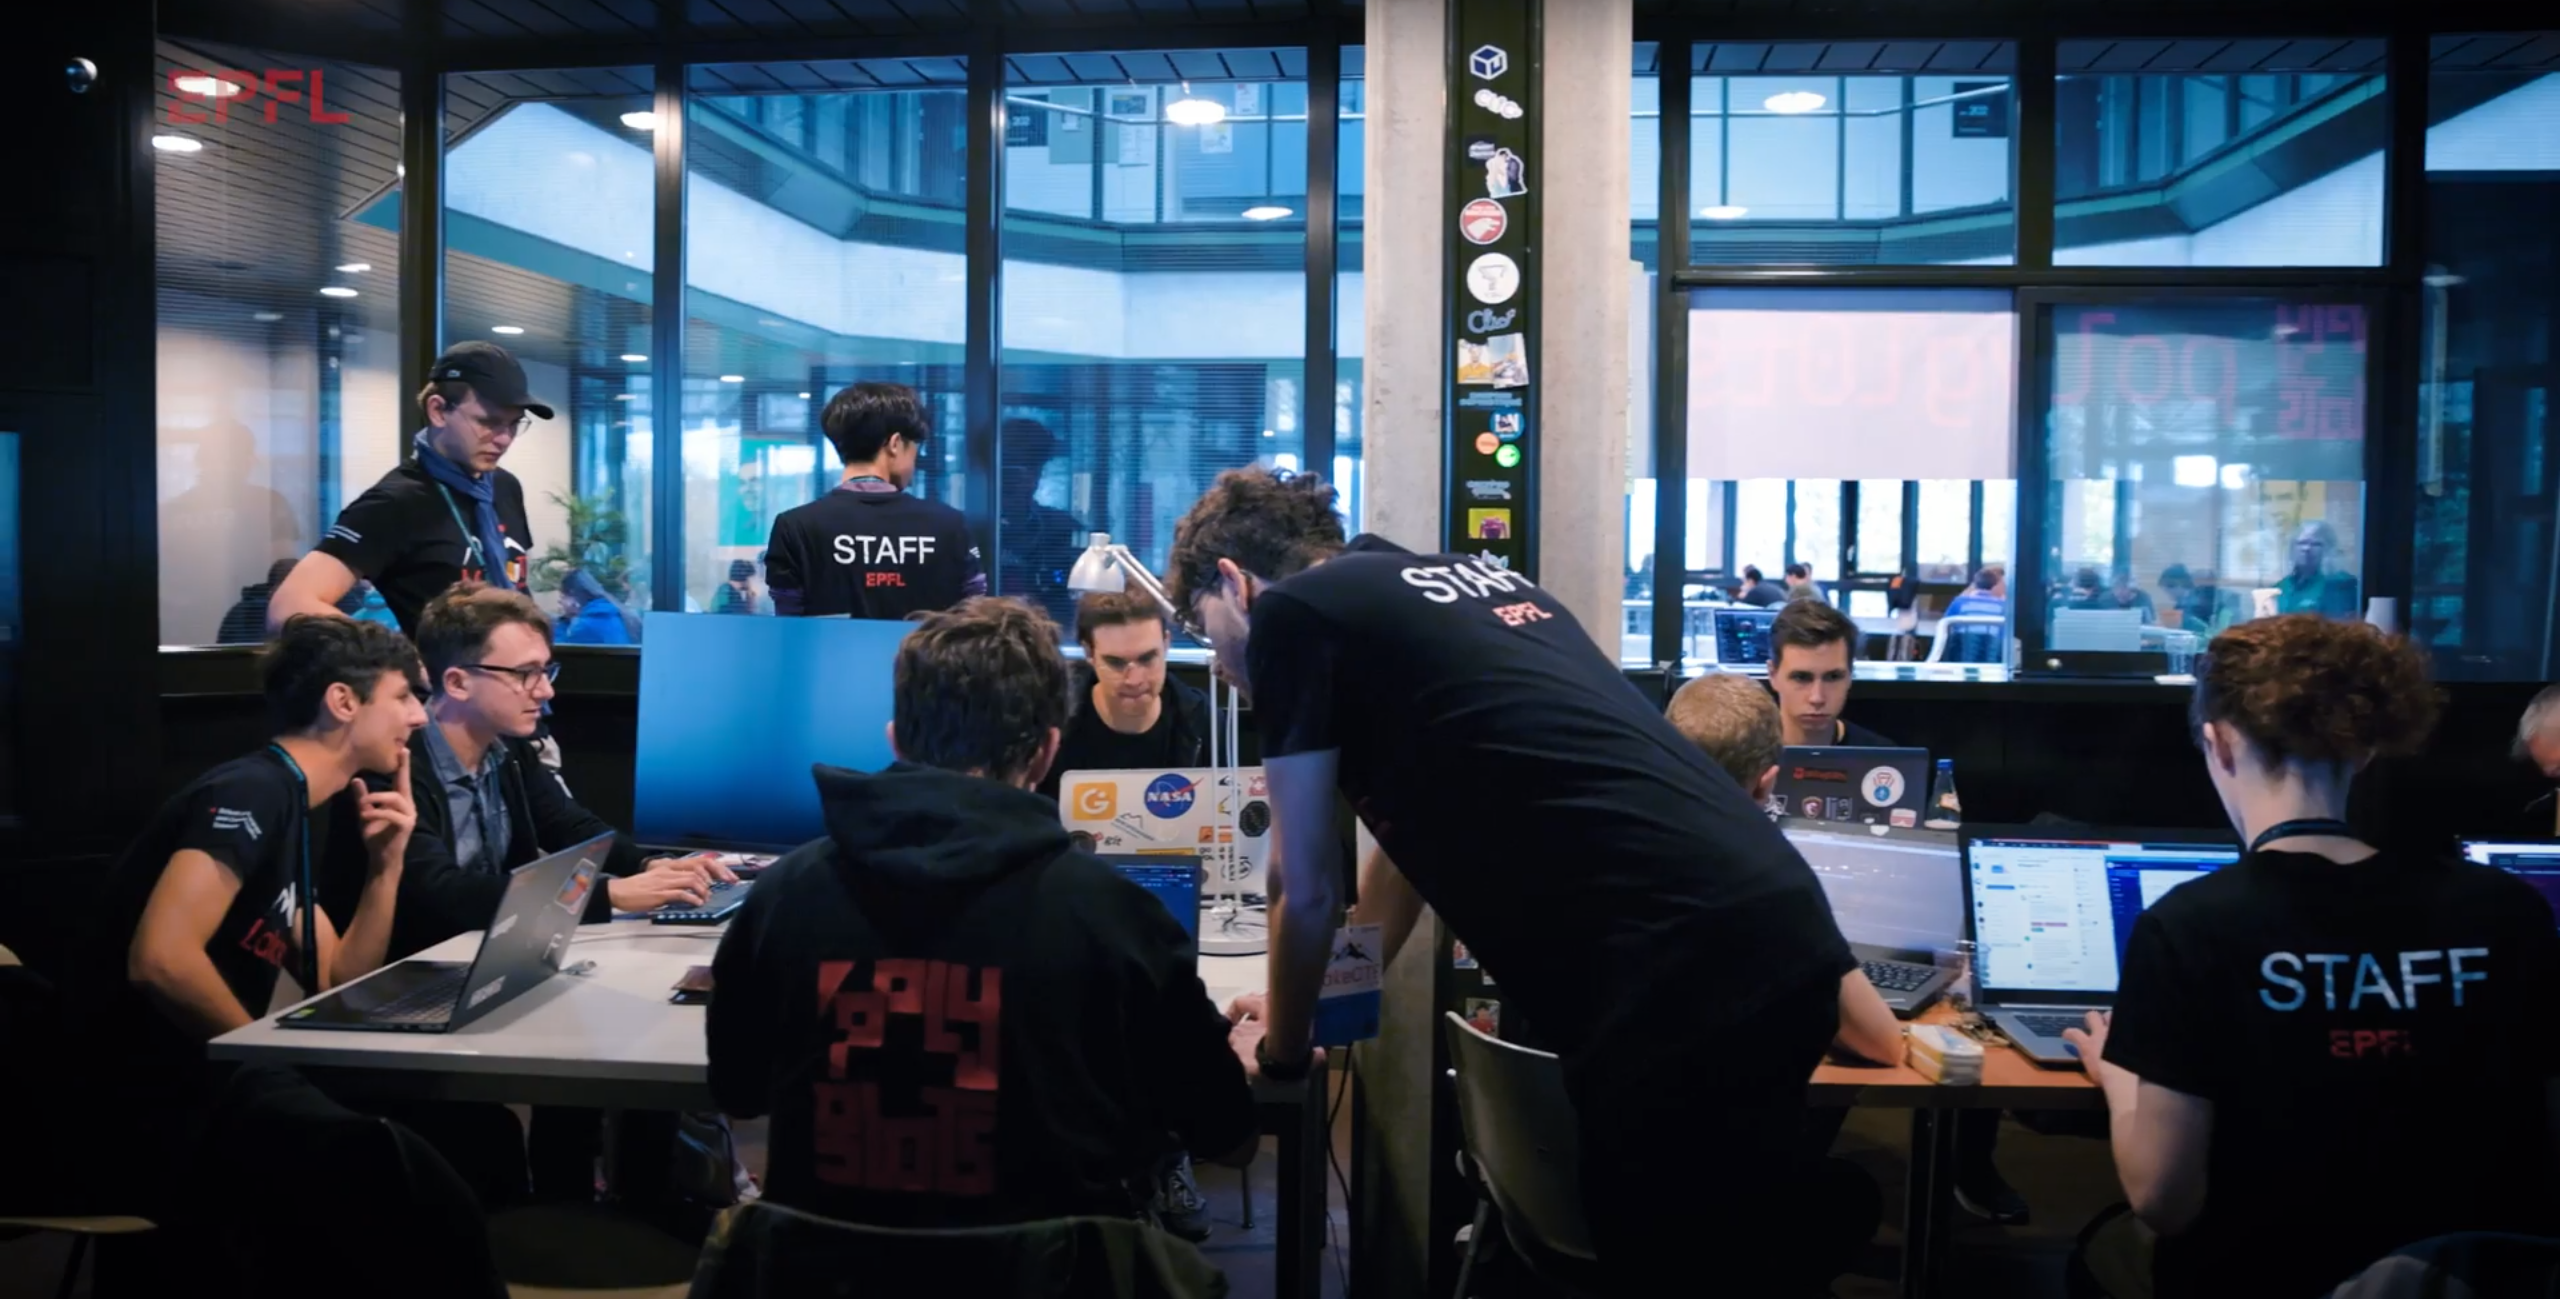
\includegraphics[scale=0.15]{./lakectf.png}};
		\end{scope}
		\node[align=center, anchor=north] at (image.south) {It's a hacking competition!};
	\end{tikzpicture}
	\end{center}
\end{frame}

\begin{frame}
	\frametitle{What even is a CTF?}
	\begin{center}
	\begin{tikzpicture}
		\begin{scope}
			\node (0,0) (image) {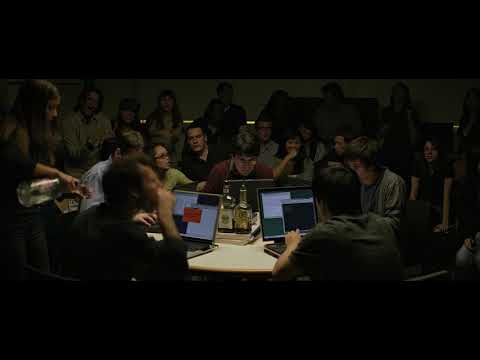
\includegraphics[scale=0.4]{./hacking.jpg}};
		\end{scope}
		\node[align=center, anchor=north] at (image.south) {Just like that scene in \textit{The Social Network}
		\\ but it's for real and people don't get drunk so easily};
	\end{tikzpicture}
	\end{center}
\end{frame}



\begin{frame}
	\frametitle{What even is a CTF?}
	\begin{itemize}
		\item CTFs are team-based cybersecurity competitions, often involving real-world attacks
        \item You score points by \emph{capturing the flag} of a given challenge, where the flag is a secret string hidden from you
	\end{itemize}
	\pause
	Challenges are divided into many categories:
	\begin{itemize}
		\item \highlight{Pwn}: Exploit binaries or services, bypass security measures, pop shells in random people's servers.
        \pause

		\item \highlight{Crypto}: Study and break crypto protocols and implementations.
        Fun is guaranteed.
        \pause

		\item \highlight{Web}: XSS attacks, CSRF vulnerabilities, backend misconfigurations. Everything that could help you get unauthorized control over a website
        \pause

		\item \highlight{Reverse}: Break down and understand the logic of a binary. Think about old-school keygens or anything related to malware analysis.
        \pause

		\item \highlight{Stegano, OSINT, Misc}: Join the team for more information :)
	\end{itemize}
\end{frame}

\begin{frame}
	\frametitle{What even is a CTF?}
	\begin{center}
	\begin{tikzpicture}
		\begin{scope}
			\node [inner sep=0pt] (0,0) (image) {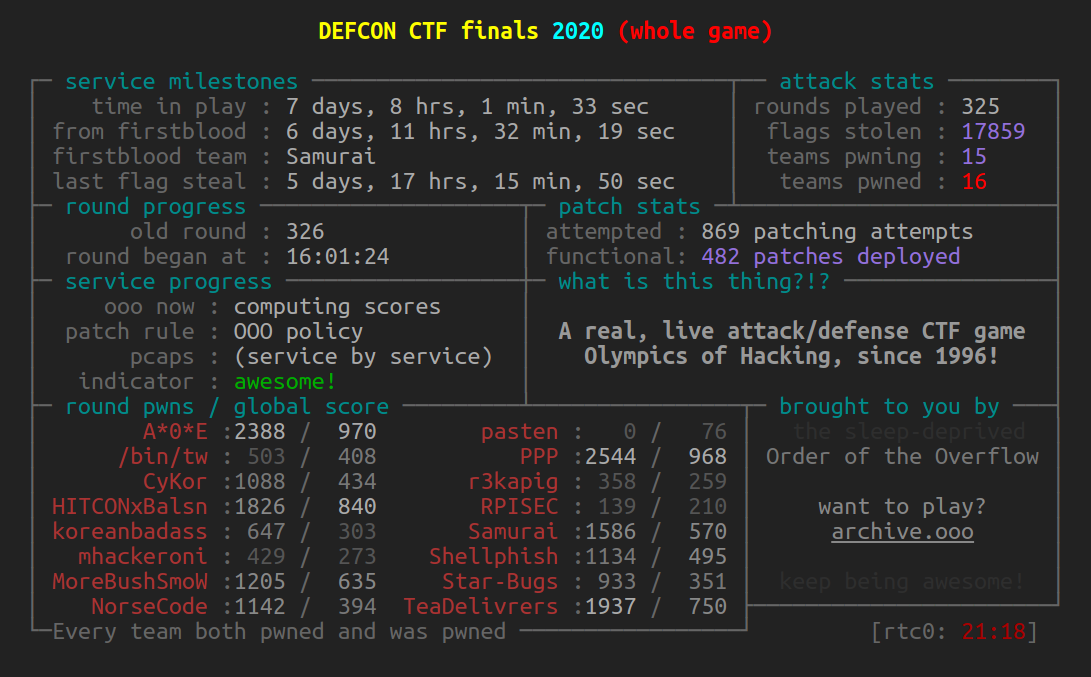
\includegraphics[scale=0.25]{./scoreboard.png}};
		\end{scope}
		\node[align=center, anchor=north] at (image.south) {Example scoreboard - Bonus points for who gets the reference :)};
	\end{tikzpicture}
	\end{center}
\end{frame}

%\begin{frame}
	%\frametitle{}
	%\begin{center}
	%\begin{tikzpicture}
		%\begin{scope}
			%\node [inner sep=0pt] (0,0) (image) {
\includegraphics[height=0.8\textheight]{./plaid.png}};
		%\end{scope}
		%\node[align=center, anchor=north] at (image.south) {Every CTF is unique};
	%\end{tikzpicture}
	%\end{center}
%\end{frame}

%\begin{frame}
	%\frametitle{Pwn chall example}
	%\begin{center}
	%\begin{tikzpicture}
		%\begin{scope}
			%\node [inner sep=0pt] (0,0) (image) {
\includegraphics[height=0.9\textheight]{./false_promise.png}};
		%\end{scope}
	%\end{tikzpicture}
	%\end{center}
%\end{frame}

%\begin{frame}
	%\frametitle{Pwn chall example}
	%\begin{center}
	%\begin{tikzpicture}
		%\begin{scope}
			%\node [inner sep=0pt] (0,0) (image) {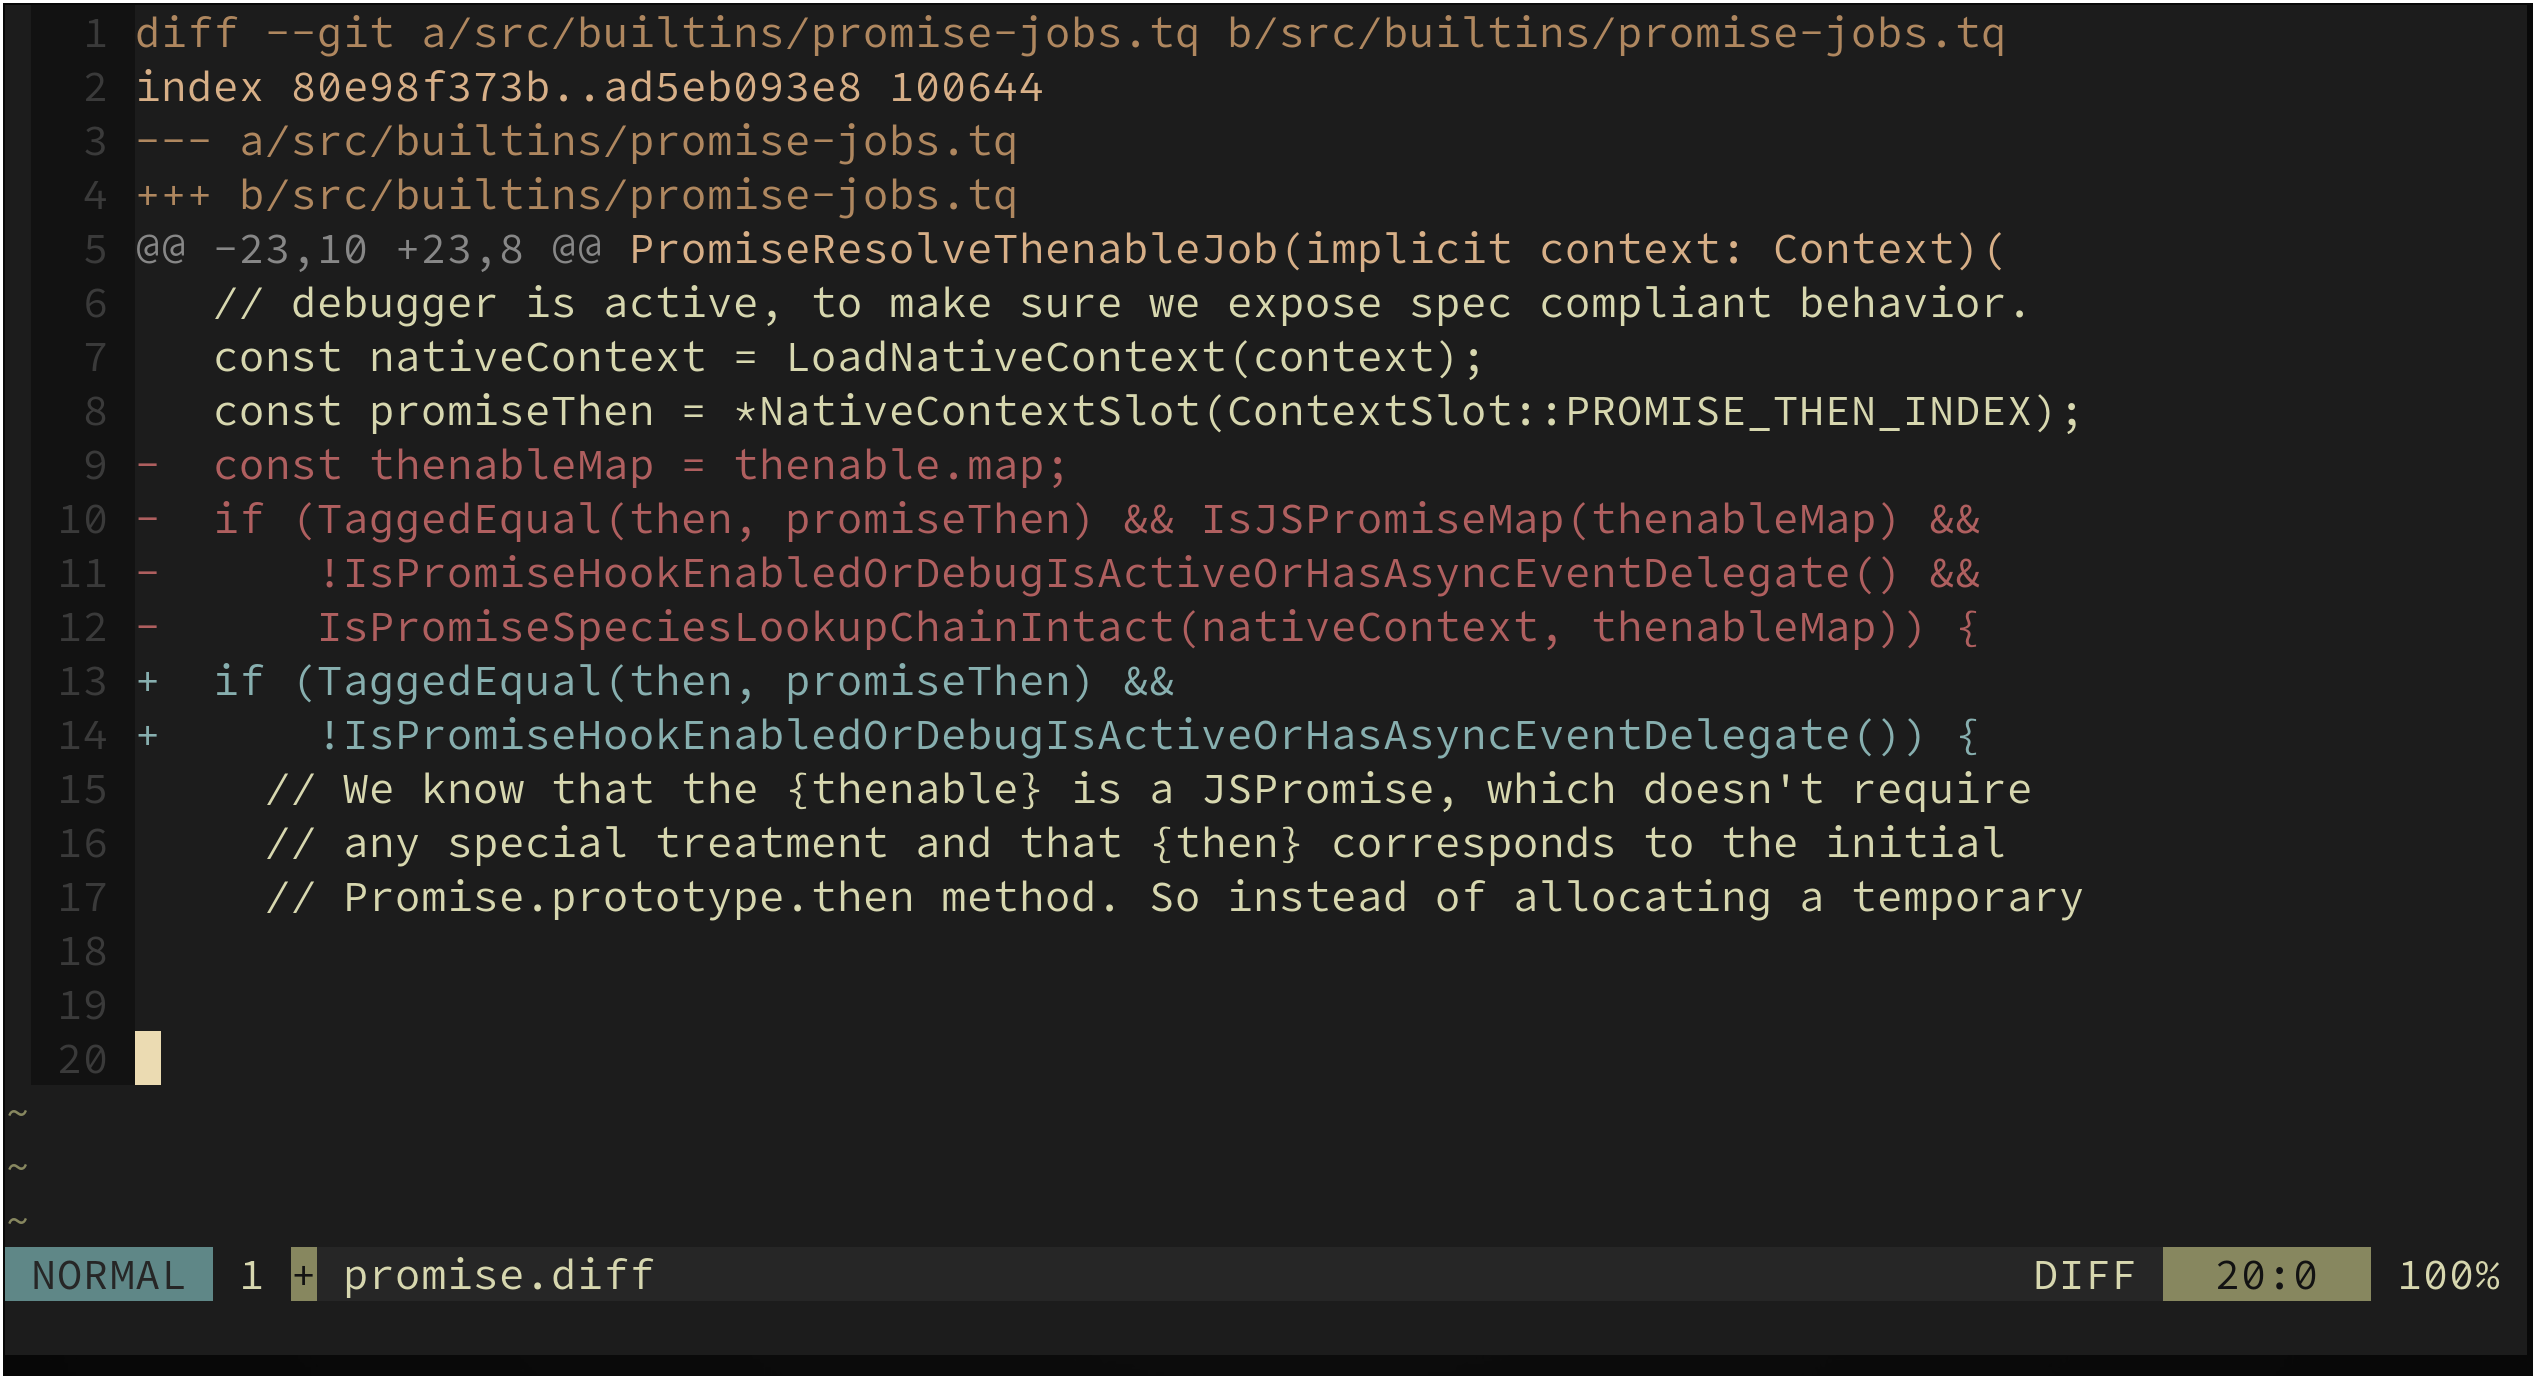
\includegraphics[height=0.8\textheight]{./chromium_diff.png}};
		%\end{scope}
	%\end{tikzpicture}
	%\end{center}
%\end{frame}

%\begin{frame}
	%\frametitle{Chromium RCE proof of concept}
	%\begin{center}
	%\begin{tikzpicture}
		%\begin{scope}
			%\node [inner sep=0pt] (0,0) (image) {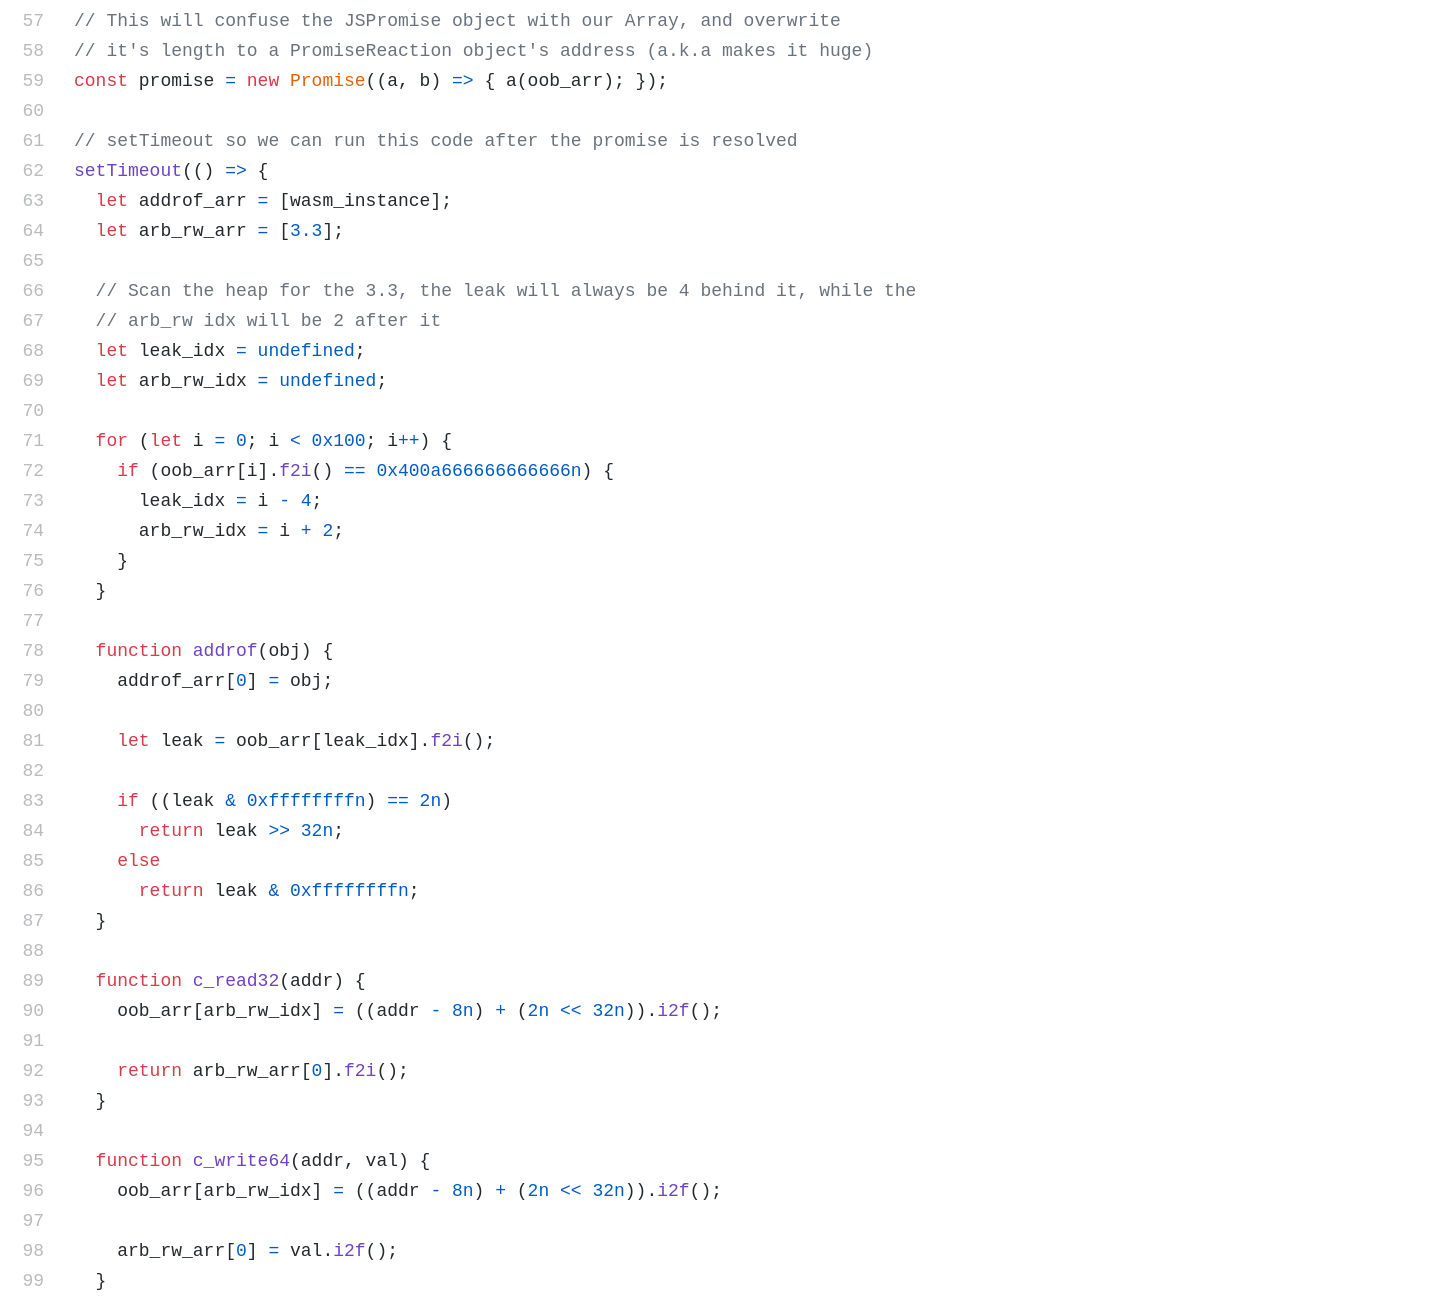
\includegraphics[height=0.8\textheight]{./promise_poc.png}};
		%\end{scope}
	%\end{tikzpicture}
	%\end{center}
%\end{frame}

%\begin{frame}
	%\frametitle{Reverse chall example}
	%\begin{center}
	%\begin{tikzpicture}
		%\begin{scope}
			%\node [inner sep=0pt] (0,0) (image) {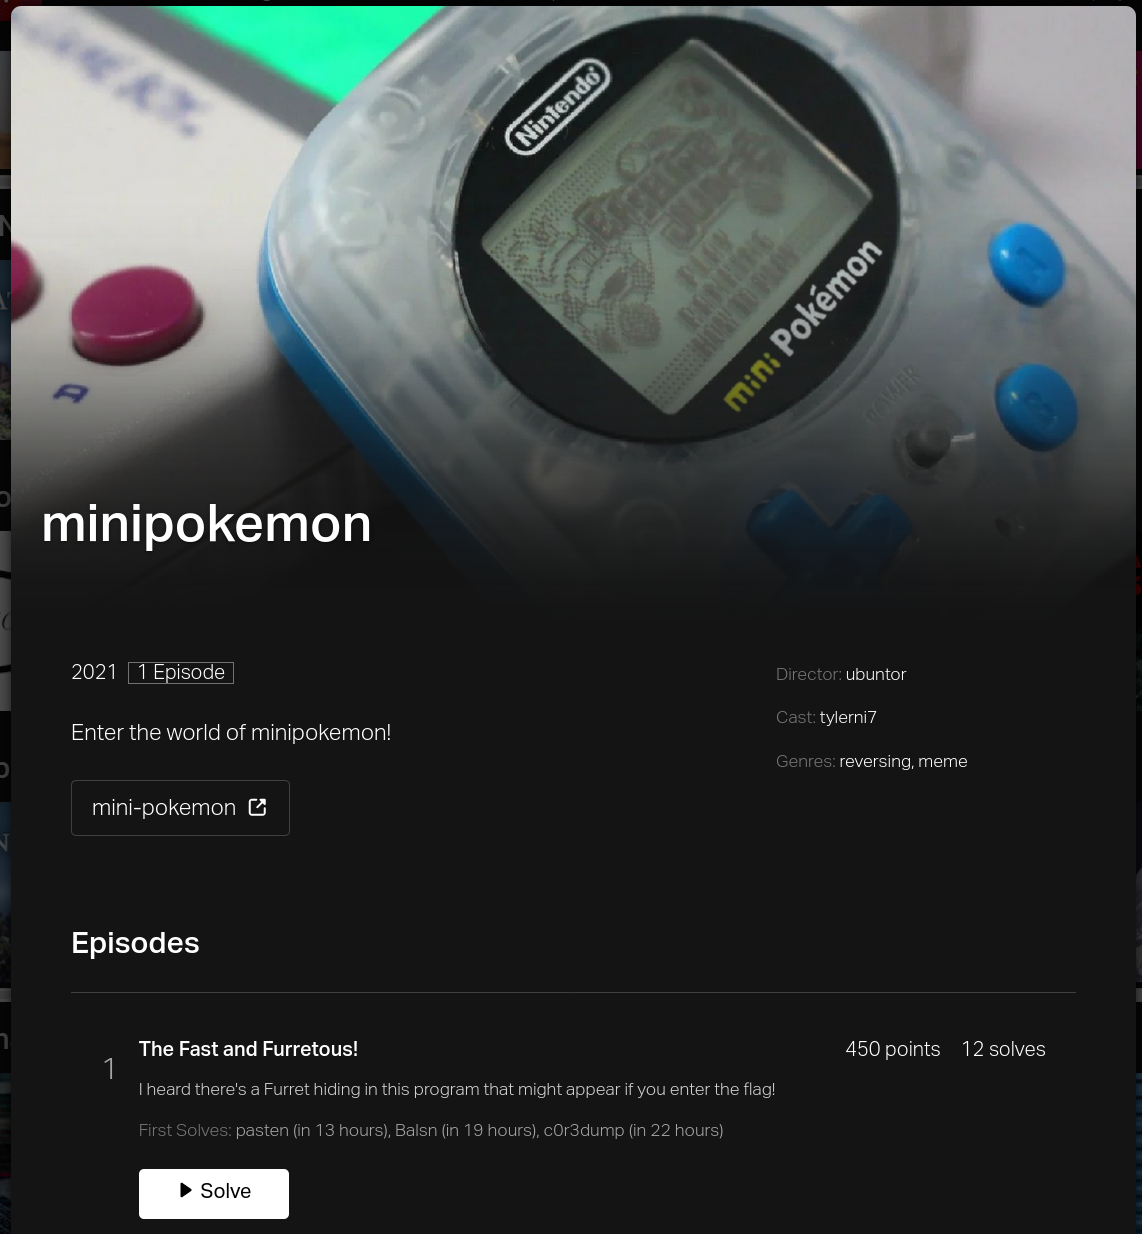
\includegraphics[height=0.8\textheight]{./pokemini1.png}};
		%\end{scope}
		%\node[align=center, anchor=north] at (image.south) {};
	%\end{tikzpicture}
	%\end{center}
%\end{frame}

%\begin{frame}
	%\frametitle{Reverse chall example}
	%\begin{columns}
		%\begin{column}{0.65\textwidth}
			%\begin{itemize}
				%\item Pokemini
				%\item Forgotten 8 bit architecture from 2001
				%\item Barely 10 games released overall
			%\end{itemize}
		%\end{column}
		%\begin{column}{0.35\textwidth}
		  %\begin{tikzpicture}
			%\begin{scope}
			  %\node [inner sep=0pt] (0,0) (image) {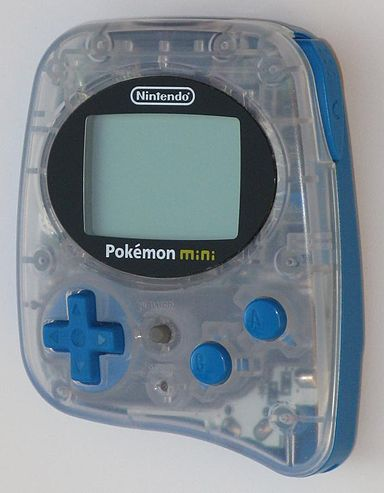
\includegraphics[width=4cm]{./pokemini5.jpg}};
			%\end{scope}
			%\node[align=center, anchor=north] at (image.south) {The pokemini in all its glory};
		  %\end{tikzpicture}
		%\end{column}
	%\end{columns}
%\end{frame}

%\begin{frame}
	%\frametitle{Reverse chall example}
	%\begin{columns}
		%\begin{column}{0.65\textwidth}
			%\begin{itemize}
				%\item Study the CPU manual to understand the instruction set
				%\item Setup the debugger and emulator environment
				%\item Write a disasm-to-IR lifter to recover CFG 
				%\item Reverse-engineer the whole thing
				%\item Re-consider all your life decisions leading to this
				%\item Figure out that the cartridge was using a version of the "masyu" puzzle
				%\item Get flag
				%\item All of the above in \textless 48 hours
			%\end{itemize}
		%\end{column}
		%\begin{column}{0.35\textwidth}
		  %\begin{tikzpicture}
			  %\node [inner sep=0pt] (0,0) (image) {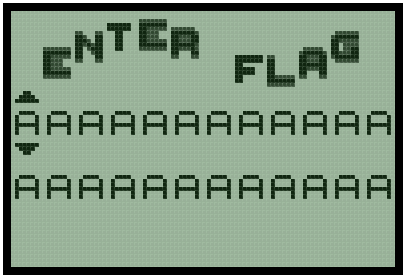
\includegraphics[width=4cm]{./pokemini2.png}};
			%\node[align=center, anchor=north] at (image.south) {Emulator screenshot};
		  %\end{tikzpicture}
		%\end{column}
	%\end{columns}
%\end{frame}


%\begin{frame}
	%\frametitle{Debugger screenshot}
	%\begin{center}
	%\begin{tikzpicture}
		%\begin{scope}
			%\node [inner sep=0pt] (0,0) (image) {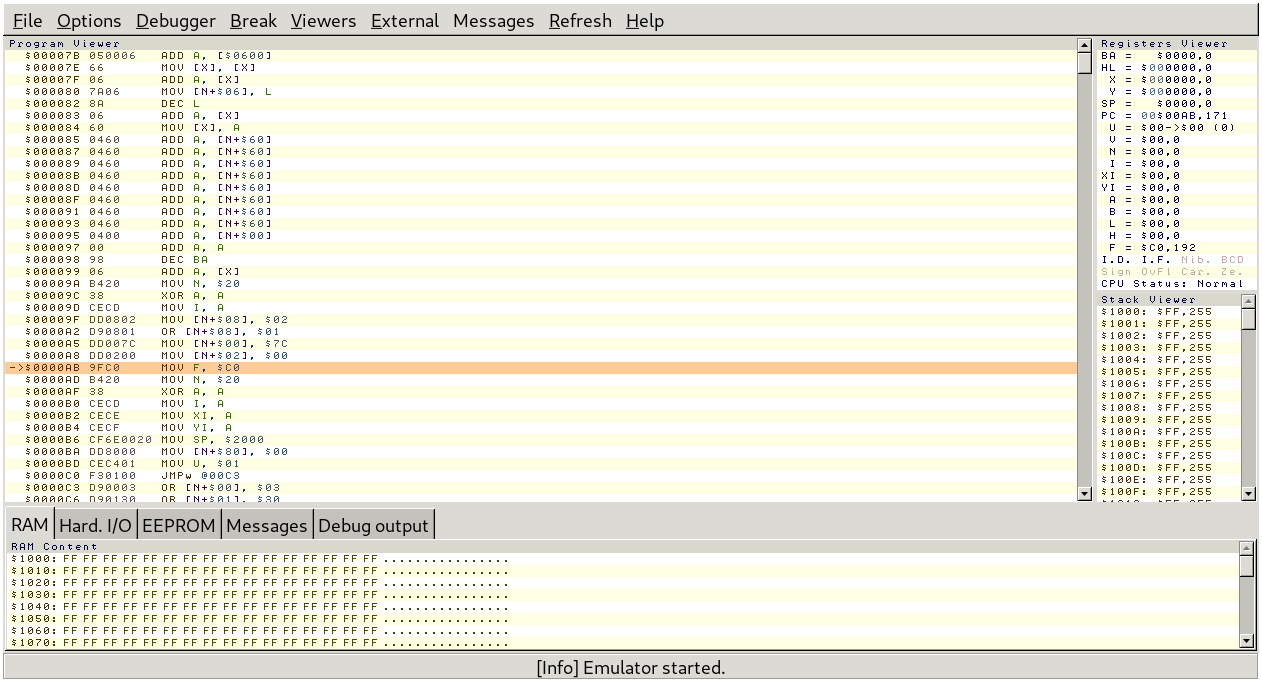
\includegraphics[height=0.8\textheight]{./pokemini3.png}};
		%\end{scope}
		%\node[align=center, anchor=north] at (image.south) {I stared at this screen for way, way longer than I'm comfortable to admit};
	%\end{tikzpicture}
	%\end{center}
%\end{frame}

%\begin{frame}
	%\frametitle{Reverse chall example}
	%\begin{center}
	%\begin{tikzpicture}
		%\begin{scope}
			%\node [inner sep=0pt] (0,0) (image) {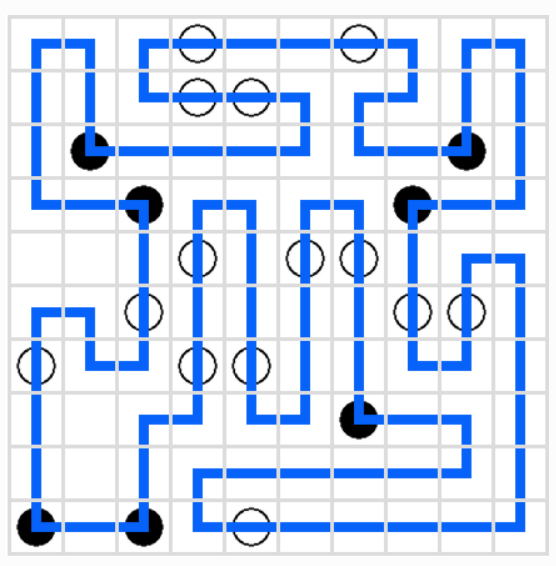
\includegraphics[height=0.8\textheight]{./pokemini4.png}};
		%\end{scope}
		%\node[align=center, anchor=north] at (image.south) {The masyu puzzle embedded in the Pokemini cartridge};
	%\end{tikzpicture}
	%\end{center}
%\end{frame}

\begin{frame}
	\frametitle{Why join us?}
	\begin{itemize}
		\item We are a strong team
		\item You'll learn huge amounts of stuff.
		\item Many security companies heavily consider CTF experience when hiring
		\item You'll meet amazing, very skilled people
		\item Join even if you are a complete noob. We have weekly meetings, tutorials, and constantly play new competitions (almost every weekend)
	\end{itemize}
\end{frame}

%\begin{frame}
	%\frametitle{Why join us?}
	%\centering
	%\begin{tikzpicture}
		%\node [inner sep=0pt] (0,0) (image) {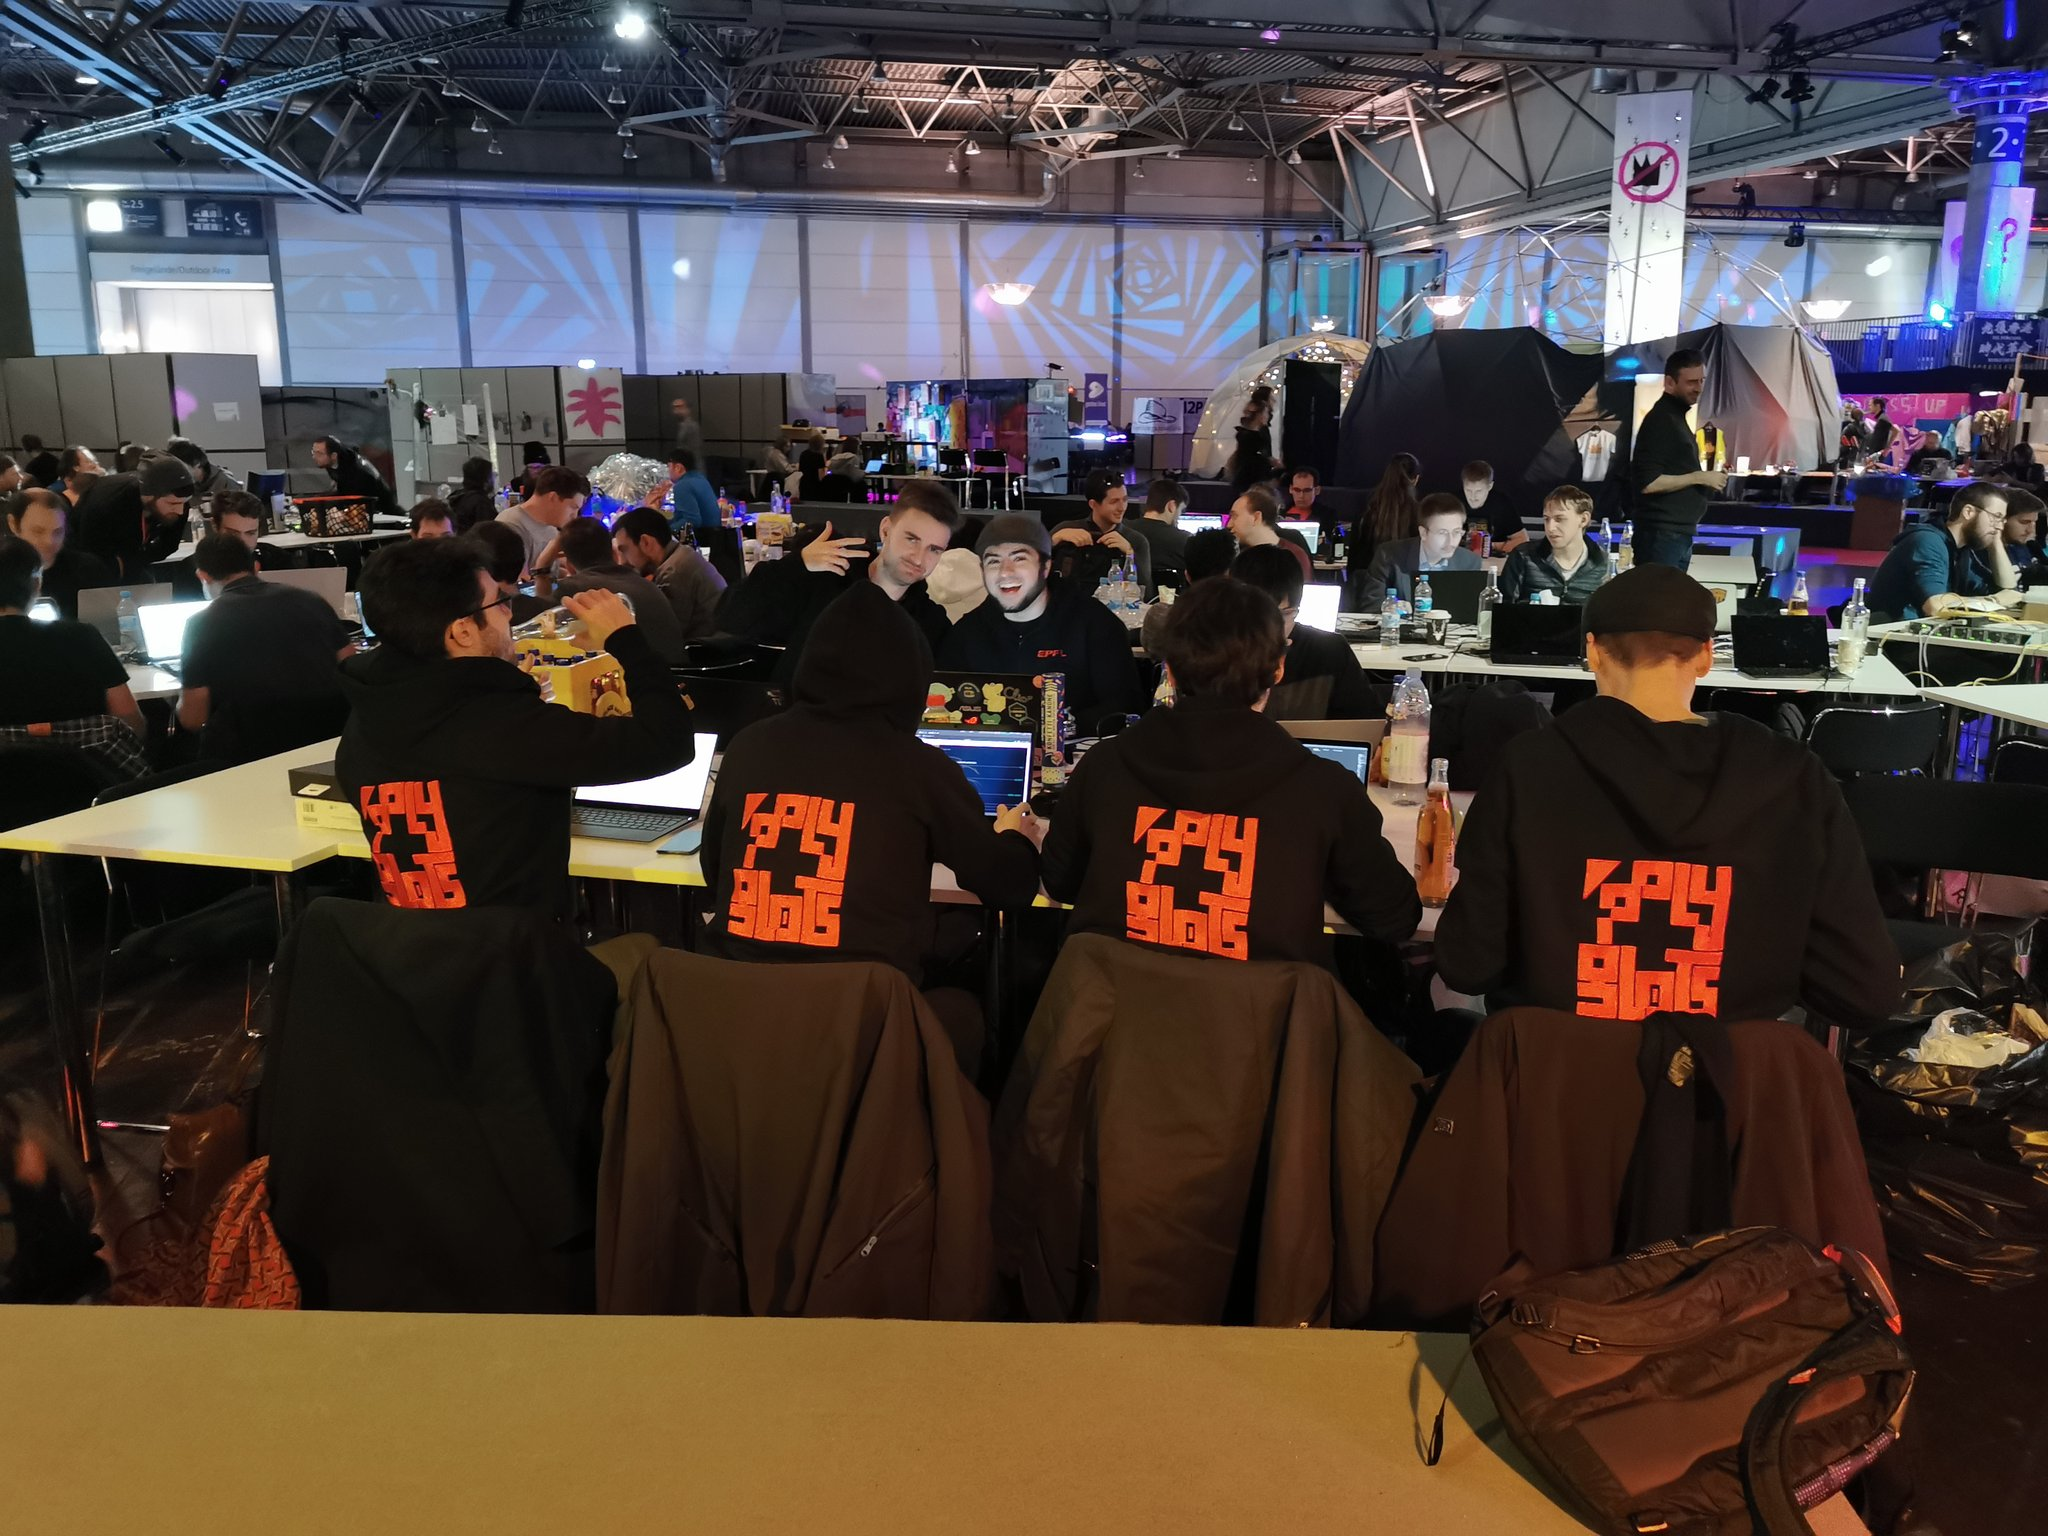
\includegraphics[height=0.8\textheight]{./CCC.jpg}};
		%\node[align=center, anchor=north] at (image.south) {We participate in cool events :)};
	%\end{tikzpicture}
%\end{frame}

%\begin{frame}
	%\frametitle{Why join us?}
	%\centering
	%\begin{tikzpicture}
		%\node [inner sep=0pt] (0,0) (image) {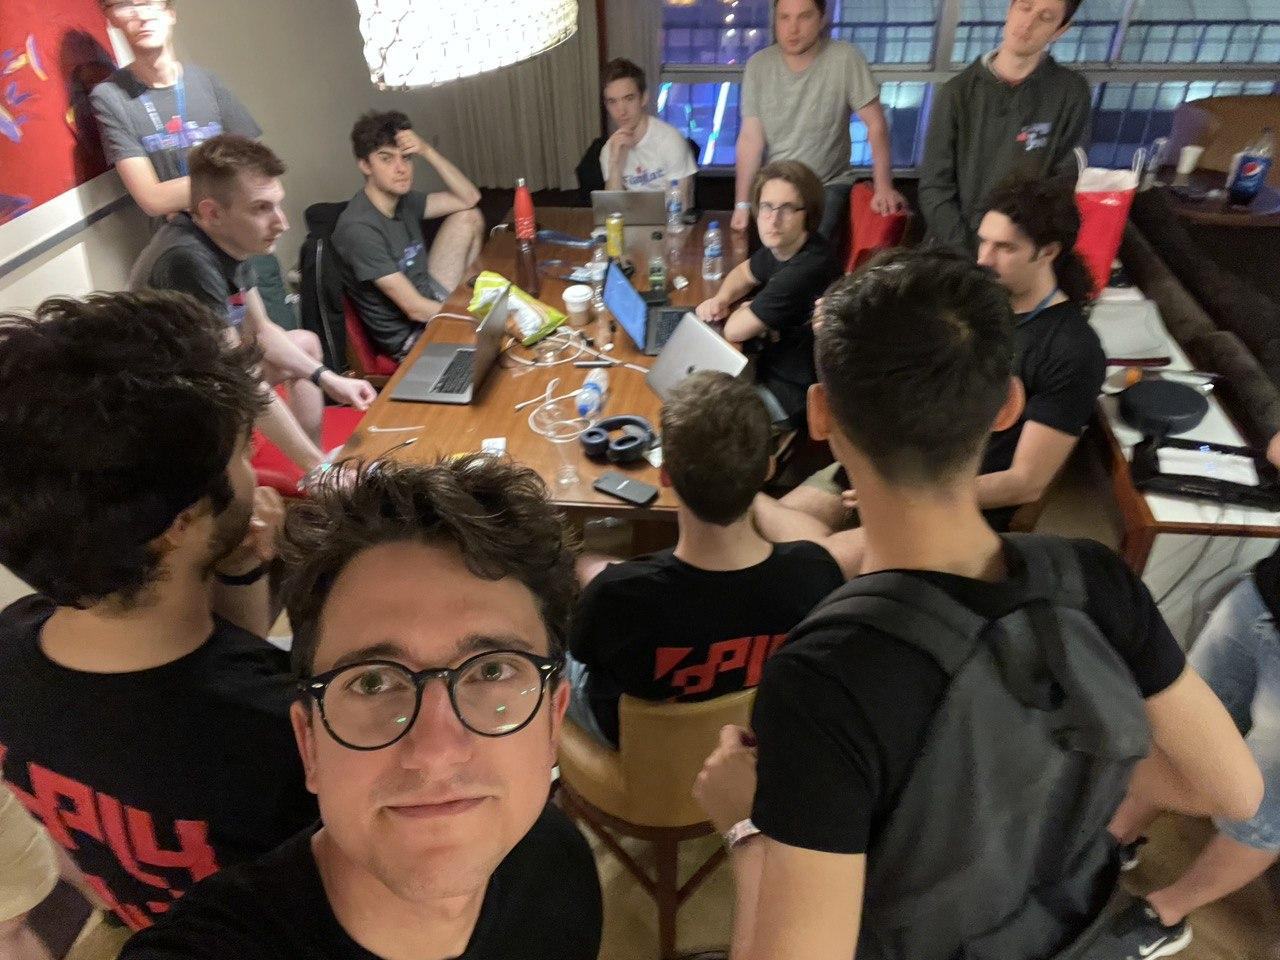
\includegraphics[height=0.8\textheight]{./real_defcon_1.jpg}};
		%\node[align=center, anchor=north] at (image.south) {DEFCON '21 - third night strategy planning};
	%\end{tikzpicture}
%\end{frame}

%\begin{frame}
	%\frametitle{Why join us?}
	%\centering
	%\begin{tikzpicture}
		%\node [inner sep=0pt] (0,0) (image) {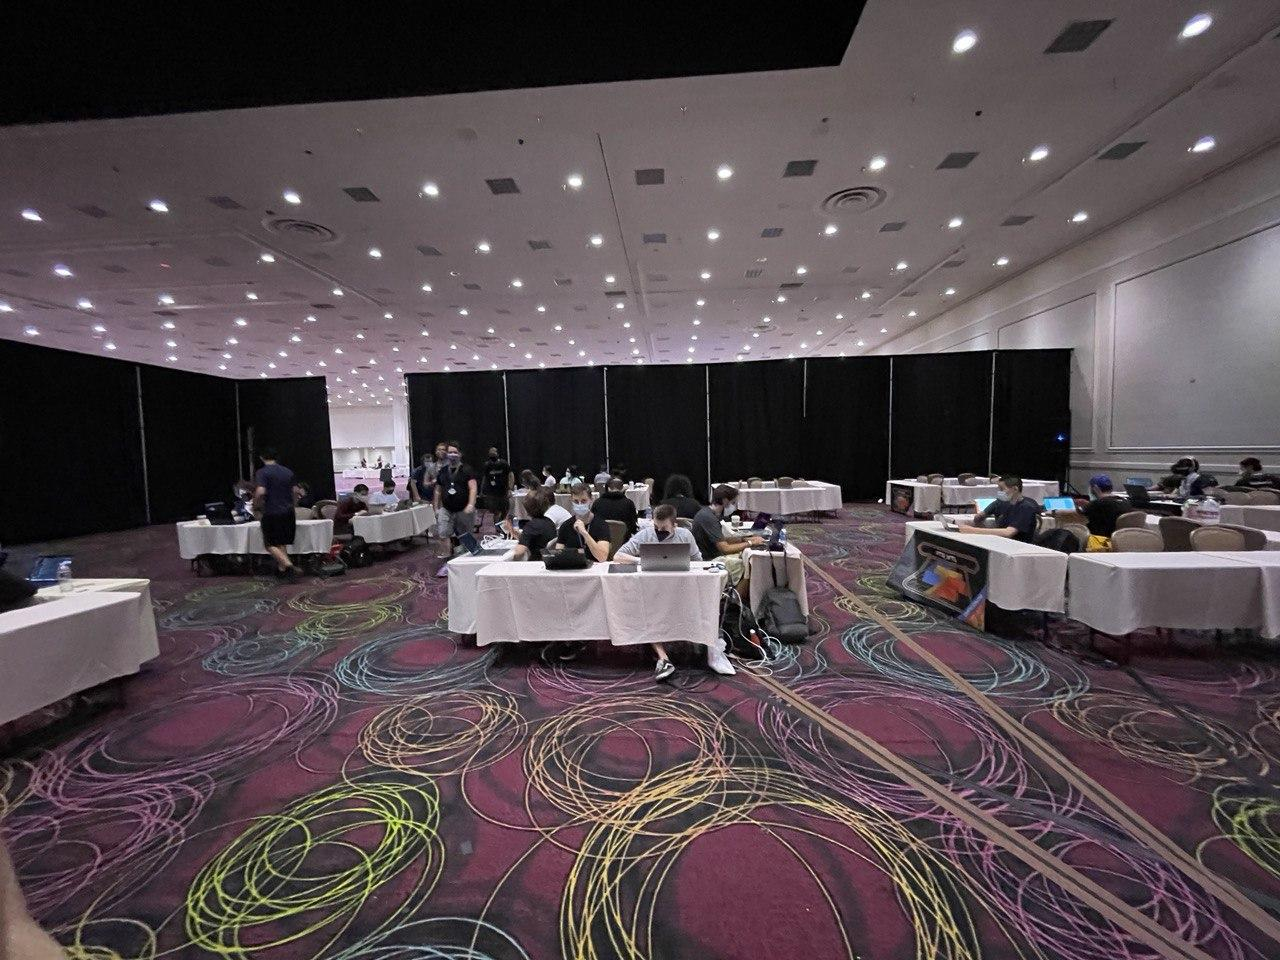
\includegraphics[height=0.8\textheight]{./real_defcon_2.jpg}};
		%\node[align=center, anchor=north] at (image.south) {DEFCON '21 - The playing stage};
	%\end{tikzpicture}
%\end{frame}

%\begin{frame}
	%\frametitle{Why join us?}
	%\centering
	%\begin{tikzpicture}
		%\node [inner sep=0pt] (0,0) (image) {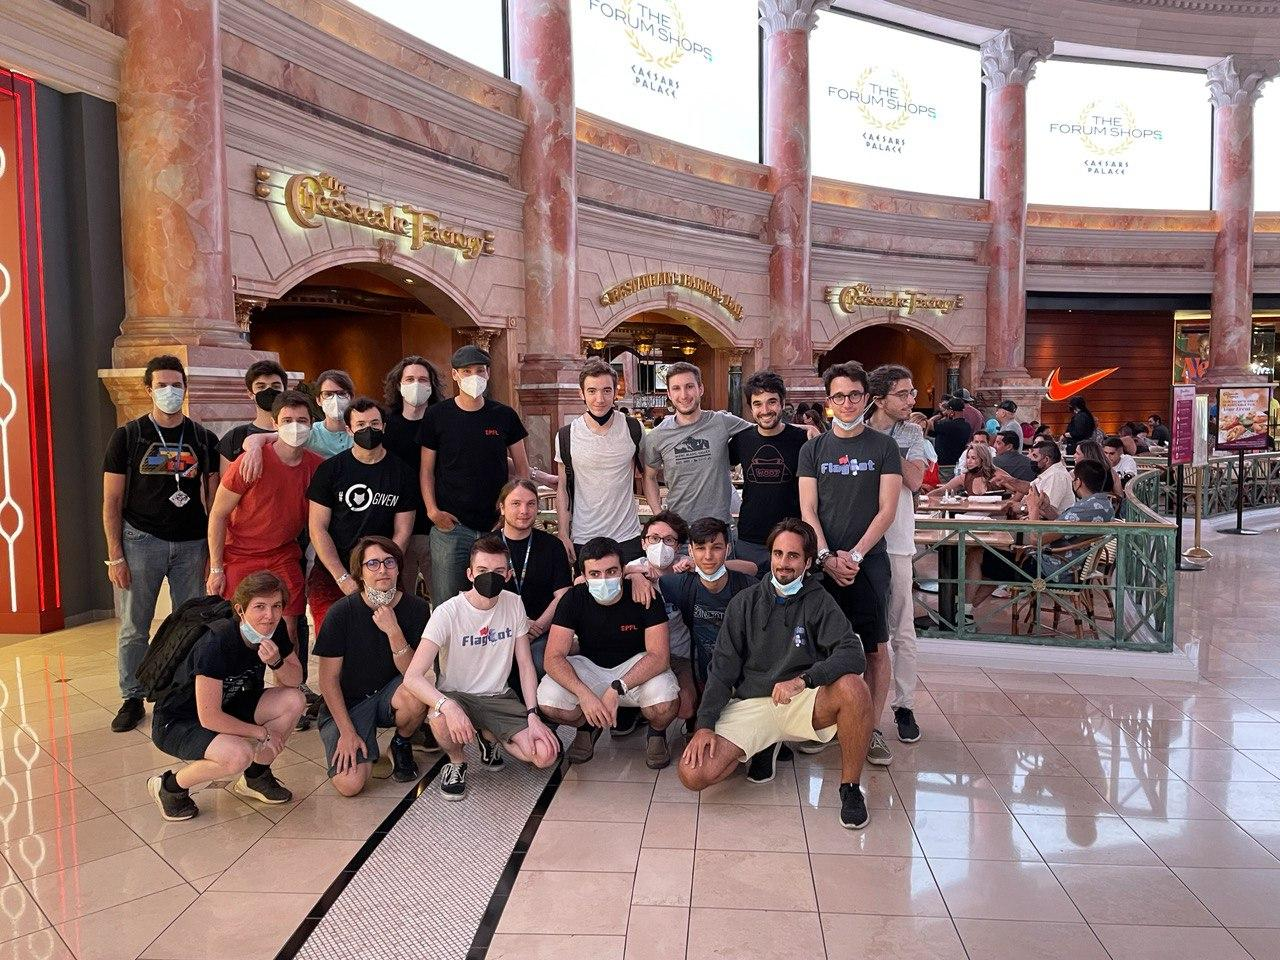
\includegraphics[height=0.8\textheight]{./real_defcon_3.jpg}};
		%\node[align=center, anchor=north] at (image.south) {DEFCON '21 - Las Vegas};
	%\end{tikzpicture}
%\end{frame}

\begin{frame}
    \frametitle{For more info}
    \begin{columns}
        \begin{column}{0.7\textwidth}
            \begin{itemize}
                % \item VIS committee and ETH's Capture the Flag team
                % \item Ranked $1^{\text{st}}$ place in Switzerland in 2019 and 2020\footnote[frame]{According to \href{https://ctftime.org/team/34878}{\UrlFont{ctftime.org}}}
                % \item Most recent: $5^{\text{th}}$ place in 0CTF (Tencent) Finals
                % \begin{itemize}
                %     \item Teamed up with polygl0ts (EPFL), the cr0wn\footnote[frame]{$1^{\text{st}}$-placed UK team}, excusemewtf? and secret club
                % \end{itemize}
                \item Visit our website: {\UrlFont{polygl0ts.ch}}
				\item Join our Discord (link in the website)
                \item Join the mailing list: send empty mail to {\UrlFont{ctf-subscribe@listes.epfl.ch}}
                \vspace{1em}
                \item CTFs usually on weekends
                \item Weekly meetings on Tuesday at 20:30 on Discord, open to anyone, some basic experience required. 
				\item Weekly tutorials on Fridays at 17:00 in BC159, oriented towards newcomers.
            \end{itemize}
        \end{column}
        \begin{column}{0.3\textwidth}
            \begin{tikzpicture}
                \begin{scope}
                  \node [inner sep=0pt] (0,0) (image) {
\includegraphics[width=4cm]{../theme/FlagbotBotOnly.png}};
                \end{scope}
              \end{tikzpicture}
            
        \end{column}
    \end{columns}
\end{frame}

\end{document}
